\section{Analyse SWOT}
\begin{figure}[H]
    \centering
    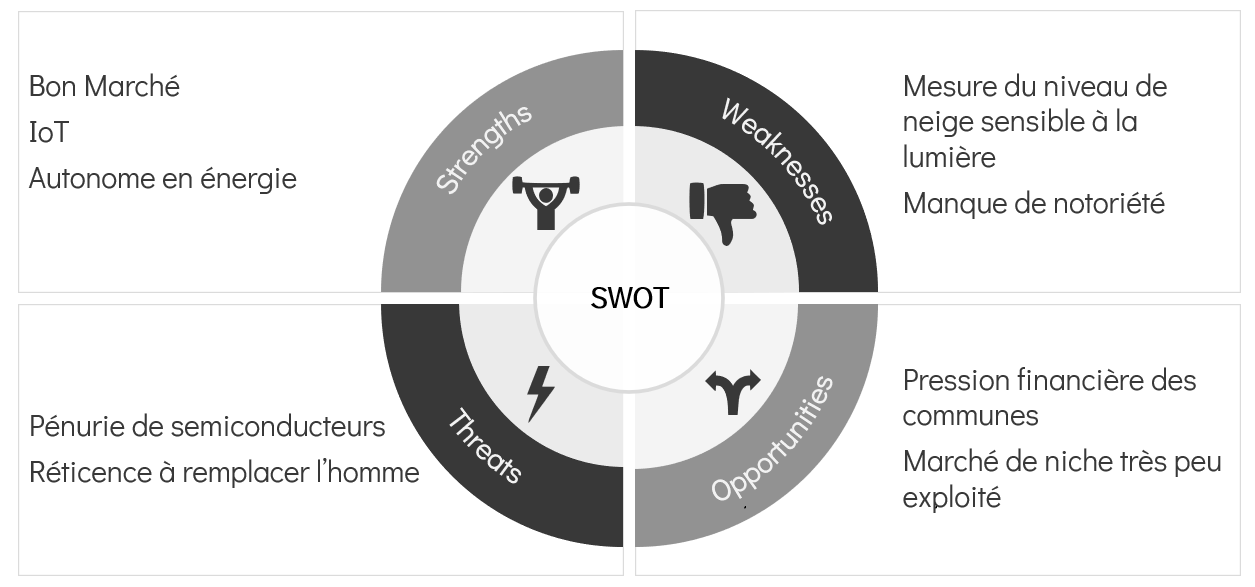
\includegraphics[width=0.85\linewidth]{Images/business/swot.PNG}
    \caption[]{Analyse SWOT}
    \label{fig:swot}
\end{figure}

\subsection{Forces}
La recherche étant réalisée par des étudiants et les composants du produit étant
bon marché, nous sommes capables de maintenir un coût bas pour un éventuel produit.

\subsection{Faiblesses}
La principale faiblesse dans notre développement, réside dans le fait que le LiDAR utilisé pour mesurer
la hauteur de neige ne fonctionne pas durant la journée.
Cependant, la surveillance des routes durant la journée n'est pas un problème et le
système remplace principalement les piquets durant la nuit.\\
Étant donné que nous sommes 3 étudiants, nous n'avons pour le moment aucune notoriété dans
le milieu et nous n'avons pas pu faire preuve de nos compétences. Les clients potentiels
risquent de se montrer méfiant à l'égard de notre produit au départ.

\subsection{Menaces}
La principale menace actuelle est la pénurie de semi-conducteurs. Si cette pénurie perdure
notre projet ne pourra pas se développer convenablement.\\
Une autre menace est la réticence à remplacer l'homme. Certaines régions comme Vex/Veysonnaz
jouissent actuellement d'un réseau du surveillance citoyenne efficace et ces régions
ne verraient pas l'intérêt d'utiliser notre produit.

\subsection{Opportunités}
La pression financière exercée sur les communes nous permettrait de s'implémenter rapidement
sur le marché. Par exemple, la ville de Sion a décidé de se séparer des services d'une entreprise
durant l'hiver 2021/2022 pour économiser. La commune d'Ayent dépense 500'000CHF chaque année pour
le déneigement et elle ne compte que 5'000 habitants.\\
De plus ce marché n'a encore été exploré. C'est donc un marché de niche sans concurrence.

\subsection{Analyse}
Pour obtenir de meilleurs résultats sur le marché, nous décidons de mettre en avant les points suivants :
\begin{description}
    \item[Bon marché - Pression financière des communes] \hfill \\
    La pression financière des communes les orientera plus facilement vers des solutions
    bon marché. 
    \item[Réticence à remplacer l'homme - Pression financière des communes] \hfill \\
    Bien que la réticence à remplacer l'homme soit présente, surtout en Valais, la pression
    financière des communes va doucement amener à supprimer le travail pénible et couteux des personnes de piquet.
    \item[Marché de niche - Faible notoriété] \hfill \\ 
    Ne pas avoir de notoriété dans un marché bien rempli est problématique. Dans un marché de niche
    tout est possible. Le fait d'être les pionniers sur ce marché palierait à notre faible notoriété.
\end{description}

\section{Stratégie adoptée}
La stratégie adoptée pour une potentielle commercialisation du produit se ferait ainsi :
\begin{itemize}
    \item LoRaSnow en format abonnement, tout inclus
    \item Le client paie une fois par année, tout le reste est pris en charge par nos soins
    \item Prix de départ de l'abonnement : 3'000CHF par appareil par année
    \item Réduction sur les abonnements par achat groupé :
    \begin{itemize}
        \item 10 appareils : 28'000CHF/an
        \item 20 appareils : 55'000CHF/an
        \item ...
    \end{itemize}
\end{itemize}
\noindent
Cette stratégie appuie bien sur le fait de rester bon marché. Le format abonnement
diminue le prix direct de l'appareil pour le client.\\
De plus, ce format permet au client de ne pas avoir à se soucier de quoi que ce soit et d'avoir
simplement un produit qui fonctionne.